\chapter{Introduction}

\section{Particulate Matter}

Nowadays, a major concern of national and international environmental agencies is to reduce and regulate the amount of particulate matter (PM) emitted in the atmosphere. \\
PM is defined by the United States Environmental Protection Agency (EPA) as a mixture of solid particles and liquid droplets found in the air \cite{epaHealthEnvironmental}. The European Environmental Agency (EEA) defines the PM as fine solid or liquid particles release into the atmosphere by processes at the Earth’s surface \cite{europaPollution}. \\
PM is responsible for reducing visibility, the reduction of photosynthesis in plants, altering soil physiochemical proprieties, and affecting meteorological processing and atmospheric chemistry \cite{mukherjee2017world}. In particular, air pollution and climate change are linked in different ways: the production of greenhouse gasses, the influence on radiative forcing by scattering or absorbing incoming radiation, and the creation of cloud condensation nuclei that affect radiative forcing and weather patterns \cite{von2015chemistry}. \\
PM can be emitted from natural sources such as dust storms, forest fires and volcanoes or by human activity, such as transportation, fuel burning and industrial processes \cite{thangavel2022recent}.
The narrow possibility to directly control natural sources of PM highlights the importance of mitigating anthropogenic emissions to reduce population health risk. \\
This is important because PM is the pollutant with the largest impact on human health \cite{harrison2020airborne} and its toxicity depends primarily on the size, shape and composition of the particles \cite{mukherjee2017world}. \\
The Global Burden of Disease Study identifies outdoor and indoor air pollution as the second leading risk factor for death and the leading risk factor for disease burden \cite{ourworldindataDeathsFrom}. \\
Especially $\text{PM}_{10}$ and $\text{PM}_{2.5}$, due to their “aerodynamic equivalent diameter” of 10 and 2.5 µm respectively, may have access to deeper regions of the respiratory tract. \\
Particles between 10 and 5 µm can deposit in the tracheobronchial tree, while those between 5 and 1 µm can reach the respiratory bronchioles and the alveoli (Fig. \ref{fig:Lungs}). Particles smaller than 1 µm can eventually be translocated into the cell tissue and circular system \cite{kim2015review}.

\begin{figure}[H]
\centering
    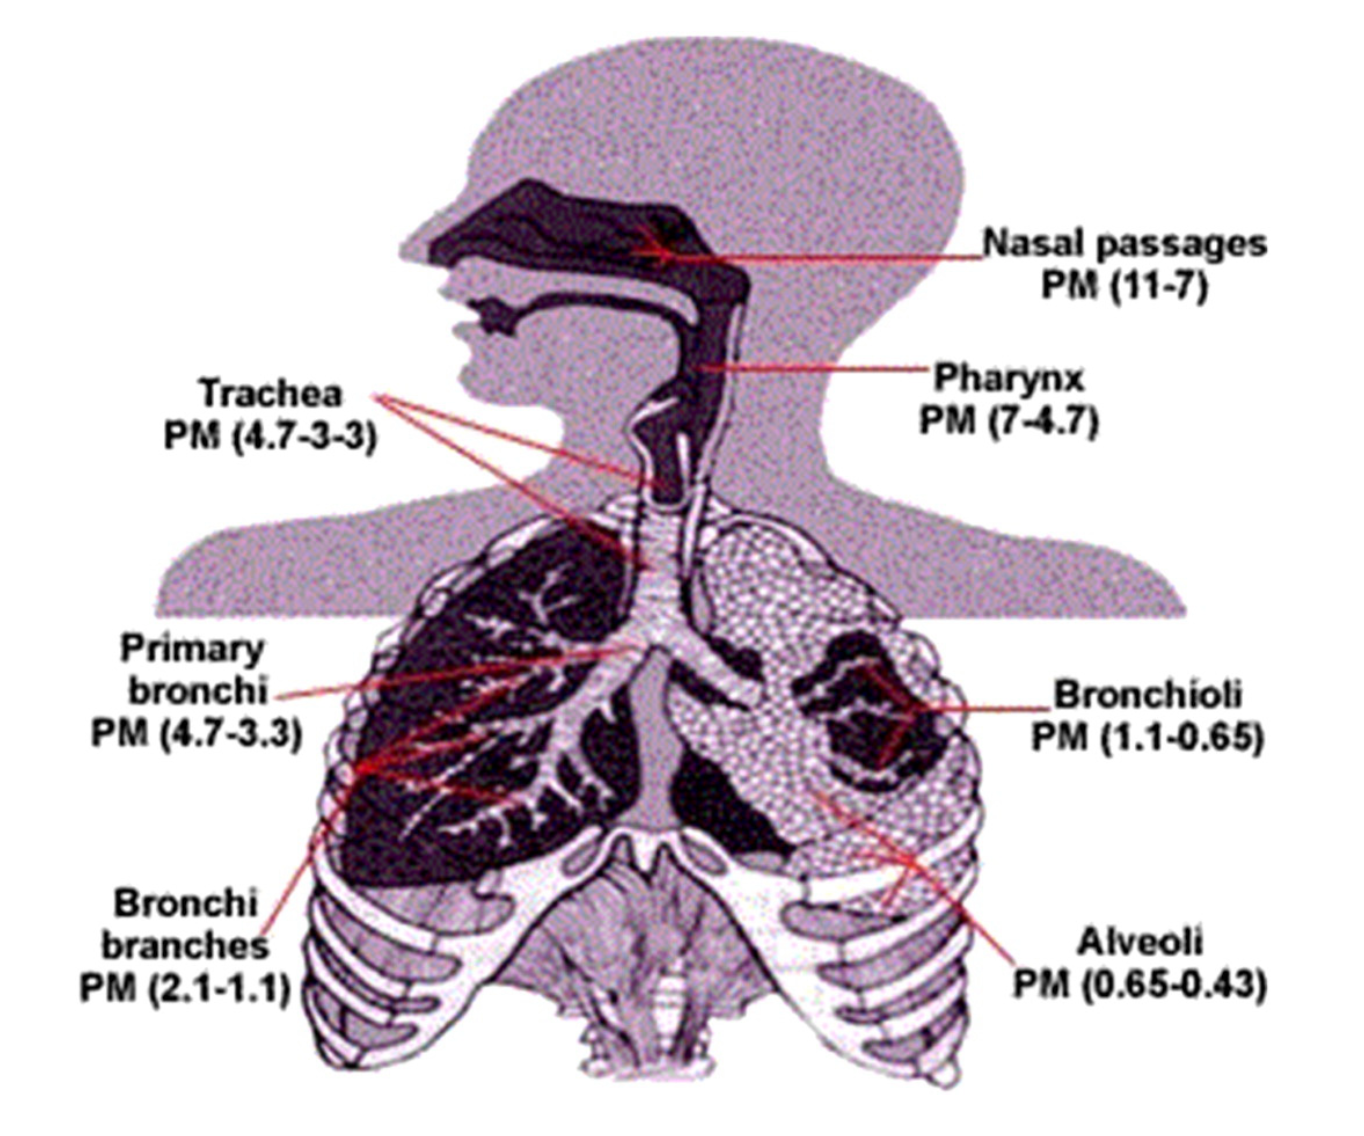
\includegraphics[scale=0.3]{images/Lungs.png}
    \caption{Potential deposition into the respiratory system of different size particles (Source: \cite{kim2015review})
}
    \label{fig:Lungs}
\end{figure}

Generally, PM enters the body through three major pathways:
\begin{enumerate}
    \item Inhalation: particles can enter through the respiratory tract. Depending on the sizing, as mentioned earlier, particles can penetrate deep into the lungs, reaching the alveolar region.
    \item Ingestion: PM can be present in contaminated food and beverage. Especially smaller particles penetrate deeper into the lungs where mucosal transport may not be as an effective removal mechanism.
    \item Dermal absorption: this is a passive process. Several factors can be considered, such as hair coverage, skin temperature and surface charge \cite{thompson2018airborne}.
\end{enumerate} 

Since inhalation is the predominant route of exposure \cite{broday2001growth}, the lungs are the primary affected organ.\\
People with chronic obstructive pulmonary disease (COPD), are the ones more sensitive to PM exposure \cite{sint2008ambient}. In particular, COPD is a progressive inflammatory condition of the lungs caused mainly by inhalation of noxious gases and PM \cite{ling2009particulate}.\\
The World Health Organization defined COPD as the third leading cause of death in 2019 \cite{whoChronicObstructive}.
Apart from inflammation, endotoxin effects, stimulation of capsaicin/irritation receptors autonomic nervous system activity and reactive oxygen species (ROS) production are observed. The latter process receives more attention \cite{li2008role}.\\
In particular, $\text{Fe}^{3+}$ can be reduced into $\text{Fe}^{2+}$ after entering the cells, which can then lead to the generation of ROS via the Fenton reaction and lipid peroxidation \cite{cory2019impact}. \\
Oxidative stress can also impact allergic inflammation, induce acute asthma exacerbations and production of antigen-inducted airway hyperactivity \cite{li2003particulate}.\\

The heart is another organ that can be directly affected by PM exposure. In particular, two different pathways have been shown: direct, especially for $\text{PM}_{2.5}$, which can traslocate directly into the bloodstream, and indirect, in which systemic inflammation poses a risk for atherosclerosis progression, increase of blood coagulability and leads to endothelial disfunction and myocardial ischemia \cite{du2016air}.
PM can also alter heart rate control by the autonomic nervous system through an increase in systolic blood pressure (Fig.\ref{fig:Heart}) \cite{fiordelisi2017mechanisms}. 

\begin{figure}[H]
\centering
    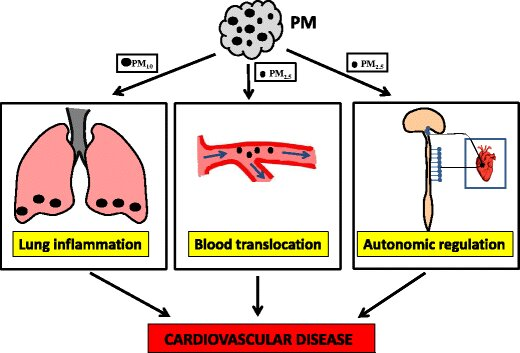
\includegraphics[scale=0.4]{images/Heart.jpg}
    \caption{Different mechanism in which PM can affect cardiovascular system (Source: \cite{fiordelisi2017mechanisms})
}
    \label{fig:Heart}
\end{figure}

Even the brain can be affected by airborne pollutant \cite{campbell2014human}, especially fine particulate matter containing heavy metals.\\
The brain is vulnerable to oxidative stress damage due to different factor: its high energy use which can generate lots of free radical, high metabolic demand and low level of endogenous scavengers, which means that is has less immune system that can neutralize free radical \cite{mohankumar2008particulate}. Ossidative stress can also influence some brain function, especially in children exposed to high levels of PM \cite{fagundes2015direct}.\\
PM can also contribute to the arise of neurodegeneration related disease such as Alzheimer’s disease (AD), Parkinson’s disease (PD) and dementia \cite{tsai2019fine}. \\
It was shown that in AD patients the levels of Fe, Cu and Zn are increased in the rims of senile plaques and Fe is high in the brain of PD patients \cite{campbell2005particulate}.\\
Inhaled PM can cross the air-to-blood tissue barrier of the lungs and reach the brain through two main pathways: directly entering via the olfactory sensory neurons or by crossing the blood-to-brain endothelial barrier \cite{hopkins2018repeated}.\\
Not only the size, but also the elements present in these particles can be problematic.
For example, the presence of Fe in PM can trigger the ferroptotic mechanism, leading to brain neuropathology \cite{cory2019impact}(Fig.\ref{fig:brain}).

\begin{figure}[H]
\centering
    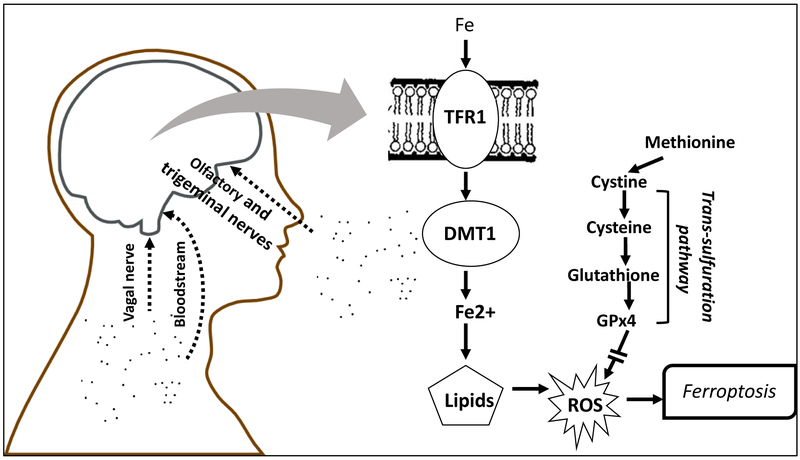
\includegraphics[scale=0.7]{images/brain.jpg}
    \caption{Diagram showing the possible pathway of ultrafine particles to the brain (Source: \cite{cory2019impact})
}
    \label{fig:brain}
\end{figure}

All this evidence proves that PM is an important factor to consider when addressing human health. Throughout their lives, people are continually exposed to PM, which can lead to a deterioration in quality of life. 
The focus on studying the PM characteristic can help understanding its nature and how it can interact with human body. \\
Considering now the area where most of the people live, it is inevitable to think about cities and their principal sources of PM. \\
Large urban areas are characterized by high pollutant emission rates due to the concentration of numerous human activities \cite{pandis2016urban}. \\
Traffic emissions are one of the major contributor to total PM \cite{pant2013estimation}, so focusing a significant portion of attention on particles emitted by vehicle circulation is warranted. \\

Generally, particles emitted from traffic are categorized into two main groups: exhaust emission from incomplete combustion and non-exhaust emission generated by wear and tear of vehicles and road surfaces \cite{grigoratos2015brake}(Fig.\ref{fig:emissions}).

\begin{figure}[H]
\centering
    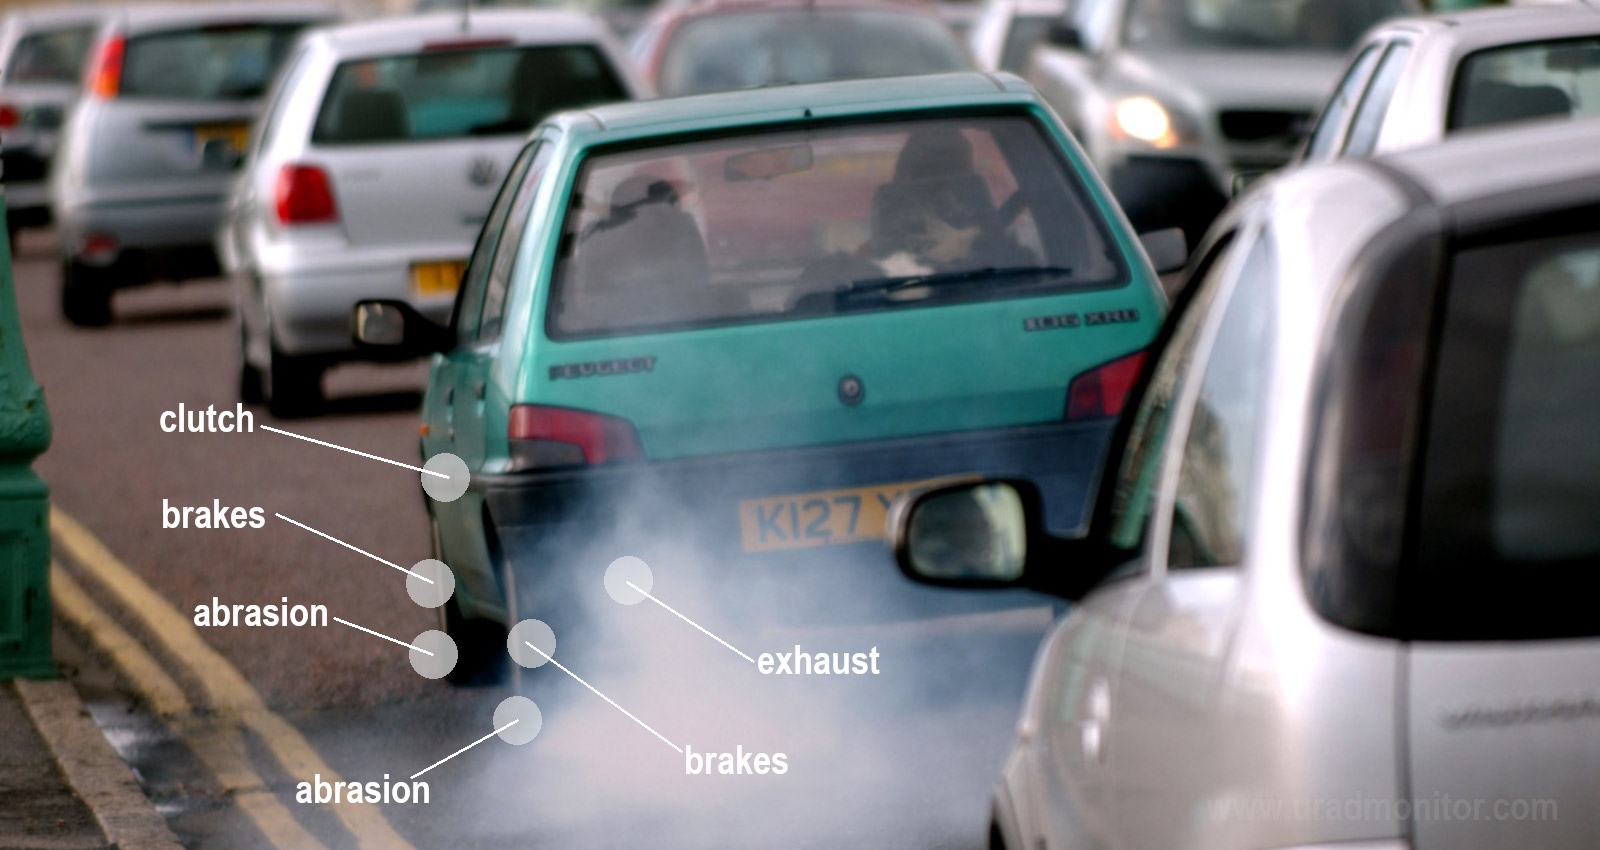
\includegraphics[scale=0.22]{images/emissions.jpg}
    \caption{Exhaust emissions resulting from the fuel combustion and non-exhausted emissions resulting from the wear and friction of varied surfaces (Source: Global Environmental Monitoring Network, 2023).
}
    \label{fig:emissions}
\end{figure}

It was proved that up to $70\%$ of brakes debris material becomes airborne as PM \cite{mulani2022review}.
To control the production of PM many limits exist, regulation such as the “Euro” emissions standards for exhaust vehicles emissions. However, limitation on non-exhaust PM emissions, primarily from tire and brake wear, are less stringent \cite{piscitello2021non}. 
Some regulations incentives hybrid or electric cars (EV) purchases to address this issue. \\
It goes without saying that the generation of exhaust emissions and greenhouse gases from vehicles within the urban environment will gradually decrease with the adoption of hybrid and electric cars. \\
These vehicles require significantly less maintenance than conventional gasoline or diesel-powered cars, particularly regarding the brake system. This reduced maintenance leads to fewer particles generated from wear and tear, making hybrid and electric cars more environmentally friendly in term of PM emissions. \\
However, it was proved that, for instance, electric cars do produce zero exhaust emissions and brake wear, but at the same time, due to their weight, they produce at the end the same amount of PM as internal combustion engine vehicles (ICEV) in terms of tyre wear, road wear and resuspension \cite{timmers2018non}. \\
This highlights the need for future regulations to address non-exhaust PM emissions alongside exhaust emissions for a more comprehensive approach to air quality management on both ICEV , hybrid cars and EV. \\
In this study, we focused on non-exhaust emission because they are less analyzed pollutants. Understanding these emissions is crucial to determine whether the ecological transition to electric and hybrid vehicles can effectively reduce human exposure to PM or if there are additional factors to take into consideration. \\


\section{Brakes}
The principal differences in car brake systems will be presented in this paragraph. \\
Conventional cars rely solely on hydraulic braking systems, in which the friction between the brake pad and rotor converts kinetic energy into heat. This process generates particles due to the high temperature and component wear and tear. \\
In contrast, hybrid and electric cars utilize a regenerative braking system. During braking, the wheels transfer kinetic energy to a generator, which converts a significant portion of this energy back into electricity to recharge the battery.\\ Additionally, the generator resistance helps in slowing down the vehicle. Friction brakes are only engaged in situations requiring more forceful braking.
Thanks to the regenerative braking system electric and hybrid vehicles release significantly less PM in the atmosphere compared to conventional cars. \\
However, it’s important to acknowledge that other factors can also impact the amount of the emitted non-exhaust PM. \\
One key factor is the vehicle mass. Heavier vehicles tend to generate more particles due to the increased wear and tear of brakes. Driving style also plays a role, frequent hard braking and acceleration can increase the amount of PM emitted. Moreover deceleration rates can influence PM generation, regenerative braking can help, but very rapid deceleration events may still required the use of traditional brakes \cite{hicks2023quantifying}. \\
It is not so easy though to affirm that hybrid and electric cars produce less PM, especially since the presence of a battery can significantly increase their weight. \\
Another factor to take into consideration is the brake type. Generally, two types of brakes are used for cars (Fig.\ref{fig:brakes}):

\begin{figure}[H]
\centering
    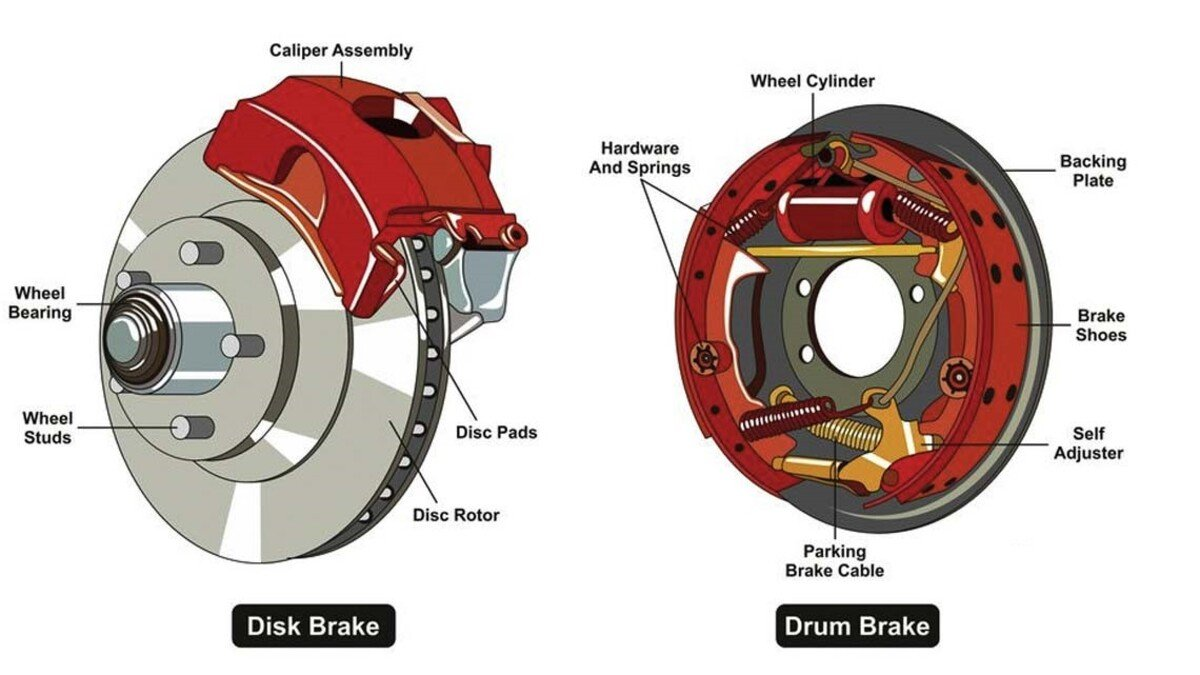
\includegraphics[scale=0.20]{images/brakes.jpg}
    \caption{Schematic representation of the two type of brakes: disc and drum (Source: Sahaj Palla, 2021).
}
    \label{fig:brakes}
\end{figure}


\begin{itemize}
    \item Disc brake, with a disc that turns with the wheel and a caliper. During braking, the caliper clamps down on the disc and the friction actions slows the wheels.
    \item Drum brake, with a hollow drum that turns with the wheel and two shoes. In this case, during braking the wheel cylinder pushes the shoes against the drum.  
\end{itemize}
Typically, modern vehicles have disc brakes on both the front and rear axles. Disc brakes provide superior stopping power and heat dissipation compared to drum brakes, which were commonly used on the rear axels of older vehicles. In even older vehicles, drum brakes might have been present on all four wheels. \\

During braking, a significant portion of the vehicle weight transfers to the front wheels. Front brakes handle about $70\%$ of a car’s total braking PM \cite{grigoratos2015brake}.
The composition of brakes pads is a critical factor, especially when considered in terms of the impact on human health. Typically, the formulation of brakes contains various heavy metals that can be harmful if inhaled or ingested in excessive amounts.
These heavy metals are present because brake pads are composed of a complex mixture of materials, each playing a specific role, such as:
\begin{itemize}
    \item Reinforcing fibers: provide structural integrity and stability. They are usually made of copper fibers, steel, brass, glass and carbon fibers.
    \item Fillers: improving thermal proprieties, noise dampening and reduce manufacturing costs. They are made of barite, potassium titanite, magnesium and chromium oxides.
    \item Abrasives: increasing friction and keep the breaks steady. They are made of zircon, quartz, aluminium and iron oxides.
    \item Lubrificants: minimize friction between the pad and the rotor. They are usually made of graphite.
\end{itemize}

Particles produced by braking often contain toxic metals like Fe, Ni, Cr, and Cu, which can generate harmful ROS. Additionally, research suggests that a higher proportion of Al in $\text{PM}_{2.5}$ can increase mortality rates \cite{kelly2012size}. \\
However, the specific composition varies significantly between manufactures and the materials and proportions vary depending on the characteristic and required performance. \\
Considering brake pad dust as a non-exhaust emission potentially harmful to humans, we can understand the danger it poses not only as a foreign body, but also due to the individual elements themselves. \\
Generally, Fe is considered the primary element in non-exhausted emissions because disc brakes are typically made of grey cast iron \cite{zemlik2022case}. \\
The wear during braking is severe, with the consequence of forming a large number of particles between the contact surfaces of friction pairs, this part is called the third body \cite{yao2023influence}. \\

Research has shown that magnetite is the primary component of friction films formed during braking. Its presence in the third body is attributed to the tribochemical oxidation of steel and iron as well as the transfer of pre-existing magnetite from the brake pad formulation \cite{yao2023influence}. \\
Furthermore, magnetite association with other elements such as Al, Ti, Ni and Pt might further elevate its toxicity \cite{ripley2024within}.
Additional research indicates that around 400°C, both magnetite and maghemite synthesized on the friction layer. As temperature reach 600°C, hematite may also be present \cite{hagino2023iron}.
Due to their formation during braking, these minerals can become dispersed in the air and inhaled by humans. This raise concerns about their potential accumulation in various organs. \\
Another concern is graphite, a common component in brake pads for lubrification and reinforcement.
Studies indicate that graphite can induce cell death (apoptosis) in lung cells \cite{zendehdel2023human}. \\ 
The combined presence of graphite with metal particles, known to trigger inflammatory response, could potentially exacerbate these effects. \\
Cu, for instance, is a common material used in brakes due to its ability to mitigate thermal fade and conductivity \cite{lee2013friction} \\
While essential for brain function, can become detrimental at high levels. Its strong redox potential can lead to oxidative stress and contribute to brain disease \cite{an2022role}, but can be also harmful to aquatic organisms \cite{lee2013friction}. \\

Nowadays, researchers are increasingly focused on substituting conventional materials, used in brakes formulations, with more environmentally friendly alternatives. For instance, significant efforts are being directed towards the use of natural fibers as reinforcement in composites \cite{hemanth2023eco} and the development of eco-friendly coating solutions to enhance the protection of automotive grey cast iron brake disks \cite{wank2023environmentally}. \\
These advancements not only aim to reduce the environmental impact but also to improve the performance and durability of automotive components.



\section{Experiment}

This study aims to characterize brake dust from different vehicles types using various techniques.
The characterization will encompass both chemical and morphology (shape and size) of the powders. \\
This analysis aims to identify the primary constituents of friction particles generated during braking and investigate potential variations between different vehicle types. \\
A dissolution test will then be conducted to investigate how these brake dust particles might interact with simulated biofluids, specifically a brain-like environment. \\
The selection of car types aimed to achieve a variety of vehicles classes, thereby considering the key parameters that influence brake dust generation. This variation included differences in engine type and weight. \\
In particular, 5 cars were taken in consideration: 
\begin{itemize}
    \item 3 conventional cars, Fiat Panda 169 (800kg), Fiat 500L (1250 kg), Fiat 500X (1300 kg).
    \item 1 liquefied petroleum gas car (LPG), Ypsilon Lancia (1040 kg). \\
    \item 1 hybrid car, Corolla Toyota (1400 kg).
\end{itemize}

For each car the powders were collected on the surface of the caliper for the disc brakes and from the shoes for the drum ones. Both anteriors and posteriors wheels were sampled. \\
EV were not included in this study due to the difficulty in obtaining a representative sample, as they are less readily available.

  









